\section{Der Dreisatz – Dein Werkzeug für Verhältnisse}

Der Dreisatz ist eines der ersten mathematischen Werkzeuge, mit denen du lernst, Beziehungen zwischen verschiedenen Mengen zu berechnen. Er begegnet dir oft im Alltag, auch wenn du ihn vielleicht nicht immer bewusst als 'Dreisatz' erkennst.

\begin{infoboxumgebung}{Was ist eigentlich ein Verhältnis? Und was bedeutet 'proportional'?}
Stell dir vor, du bäckst einen Kuchen. Im Rezept steht: 'Für 4 Personen nimm 200g Mehl'. Das ist ein \textbf{Verhältnis}! Es sagt dir, wie viel Mehl du für eine bestimmte Anzahl von Personen brauchst. Wenn du für mehr Personen backen willst (z.B. 8 Personen), brauchst du auch mehr Mehl (nämlich 400g) – und zwar im gleichen Verhältnis (hier: 50g Mehl pro Person). Verhältnisse helfen uns, Mengen fair aufzuteilen oder anzupassen.

Das Wort \textbf{'proportional'} klingt vielleicht kompliziert, aber du kannst es dir auch als \textbf{'pro Portion'} vorstellen. In unserem Kuchenbeispiel ist die 'Portion' eine Person, und \textit{pro Person} brauchen wir 50g Mehl. Wenn sich also die Anzahl der Personen (Portionen) erhöht, muss sich die Mehlmenge im gleichen Maße oder Verhältnis erhöhen, damit das Rezept noch stimmt. Verdoppelst du die Personen, verdoppelst du das Mehl. Verdreifachst du die Personen, verdreifachst du das Mehl. Das ist die Kernidee hinter 'direkt proportional'.
\end{infoboxumgebung}

Der Dreisatz ist besonders nützlich, wenn zwei Größen \textbf{direkt proportional} zueinander sind. Das bedeutet, je mehr von dem einen, desto mehr von dem anderen – und umgekehrt, im stets gleichen Verhältnis.

\begin{merksatzumgebung}[Definition Dreisatz]{Was ist der Dreisatz?}
Der Dreisatz ist eine super Methode, um Aufgaben mit \textbf{proportionalen Zusammenhängen} zu lösen. 'Proportional' bedeutet: Wenn sich eine Größe verdoppelt, verdoppelt sich auch die andere. Wenn sich eine Größe halbiert, halbiert sich auch die andere. Das Verhältnis zwischen den beiden Größen bleibt immer gleich.

Mathematisch sagt man:
\[
\text{Größe}_1 \text{ ist proportional zu Größe}_2 \quad \Leftrightarrow \quad \frac{\text{Größe}_1}{\text{Größe}_2} = \text{konstant}
\]
Das Zeichen für 'ist proportional zu' ist $\propto$. Also: $\text{Größe}_1 \propto \text{Größe}_2$.

\textbf{Warum 'Drei-Satz'?} Weil man meistens in drei Schritten (Sätzen) zur Lösung kommt:
\begin{enumerate}
    \item \textbf{Was weiß ich?} Schreibe das bekannte Verhältnis auf (z.B. 3 Äpfel kosten 1,80 €).
    \item \textbf{Auf die Einheit bringen (Zwischenschritt):} Rechne aus, wie viel von der einen Größe einer einzelnen Einheit der anderen Größe entspricht (z.B. Was kostet 1 Apfel?). Dieser Schritt ist der Schlüssel!
    \item \textbf{Hochrechnen (Schlusssatz):} Rechne von dieser Einheitsgröße auf die gesuchte Menge hoch (z.B. Was kosten 5 Äpfel?).
\end{enumerate}
\end{merksatzumgebung}

Schauen wir uns das an einem klassischen Beispiel an.

\begin{beispielumgebung}[Apfelkauf]{Der Klassiker: Äpfel kaufen}
\textbf{Problem:} Wenn 3 Äpfel 1,80 Euro kosten, wie viel kosten dann 5 Äpfel?

\textbf{Lösung mit dem Dreisatz (Schritt für Schritt):}

\begin{enumerate}
    \item \textbf{Was weiß ich? (1. Satz)}
    \begin{tabular}{rcl}
        3 Äpfel & $\ entspricht $ & 1,80 Euro \\
    \end{tabular}
    Diese Information ist unsere Ausgangsbasis.

    \item \textbf{Auf die Einheit bringen (Preis für 1 Apfel) (2. Satz)}
    Um von 3 Äpfeln auf 1 Apfel zu kommen, teile ich die Anzahl der Äpfel durch 3. Damit das Verhältnis gleich bleibt, muss ich auch den Preis durch 3 teilen:
    \begin{tabular}{rcl}
        3 Äpfel & $\xrightarrow{:3}$ & 1 Apfel \\
        1,80 Euro & $\xrightarrow{:3}$ & 0,60 Euro \\
    \end{tabular}
    Also: 1 Apfel kostet 0,60 Euro. Diesen Wert (0,60 €/Apfel) nennt man auch den \textbf{Proportionalitätsfaktor}.

    \item \textbf{Hochrechnen (Preis für 5 Äpfel) (3. Satz)}
    Um von 1 Apfel auf 5 Äpfel zu kommen, multipliziere ich die Anzahl der Äpfel mit 5. Entsprechend muss ich auch den Preis für einen Apfel mit 5 multiplizieren:
    \begin{tabular}{rcl}
        1 Apfel & $\xrightarrow{\times 5}$ & 5 Äpfel \\
        0,60 Euro & $\xrightarrow{\times 5}$ & 3,00 Euro \\
    \end{tabular}
\end{enumerate}

\textbf{Antwort:} 5 Äpfel kosten 3,00 Euro.

\textbf{Kurzschreibweise (oft in der Schule):}
\begin{tabular}{rcccl}
    3 Äpfel & $\widehat{=}$ & 1,80 € & & \\
    1 Apfel & $\widehat{=}$ & 1,80 € : 3 = 0,60 € & & \small{(geteilt durch 3 auf beiden Seiten)} \\
    5 Äpfel & $\widehat{=}$ & 0,60 € $\times$ 5 = 3,00 € & & \small{(mal 5 auf beiden Seiten)} \\
\end{tabular}
\end{beispielumgebung}

\textit{Selbst-Check:} Kannst du erklären, warum der Schritt 'Auf die Einheit bringen' so wichtig ist? Was würde passieren, wenn man ihn überspringt? (Antwort: Ohne den Preis für EINEN Apfel zu kennen, wüssten wir nicht, mit welchem Faktor wir multiplizieren müssen, um den Preis für FÜNF Äpfel zu finden. Der 'Einheitspreis' ist der Schlüssel zum Hochrechnen.)

Jetzt bist du dran! Versuche, die nächste Aufgabe genauso strukturiert zu lösen.

\begin{aufgabenumgebung}{Bücherkauf}
Wenn 4 gleiche Notizbücher zusammen 10 Euro kosten, wie viel kosten dann 7 dieser Notizbücher?
Zeichne auch ein kleines Schema wie im Beispiel (mit den Pfeilen $:4$ und $\cdot7$).
\end{aufgabenumgebung}

Der Dreisatz funktioniert nicht nur beim Einkaufen, sondern auch in vielen anderen Situationen.

\begin{beispielumgebung}[Maschine produziert Teile]{Arbeit einer Maschine}
Eine Maschine produziert in 5 Stunden 200 Teile. Wie viele Teile produziert sie in 8 Stunden (angenommen, sie arbeitet immer gleich schnell)?

\textbf{Lösung:}
\begin{enumerate}
    \item \textbf{Was weiß ich?} 5 Stunden $\widehat{=}$ 200 Teile.
    \item \textbf{Auf die Einheit (Produktion in 1 Stunde):}
        1 Stunde $\widehat{=}$ 200 Teile : 5 Stunden = 40 Teile/Stunde.
        (Die Maschine schafft also 40 Teile pro Stunde. Das ist wieder unser Proportionalitätsfaktor).
    \item \textbf{Hochrechnen (Produktion in 8 Stunden):}
        8 Stunden $\widehat{=}$ 40 Teile/Stunde $\times$ 8 Stunden = 320 Teile.
\end{enumerate}
\textbf{Antwort:} In 8 Stunden produziert die Maschine 320 Teile.
\end{beispielumgebung}

Manchmal muss man ein bisschen um die Ecke denken, wie bei der nächsten Aufgabe.

\begin{aufgabenumgebung}{Autoverbrauch}
Ein Auto verbraucht auf einer Strecke von 150 km genau 12 Liter Benzin.
\begin{enumerate}
    \item Wie viel Benzin verbraucht es auf einer Strecke von 250 km?
    \item Wie weit kommt das Auto mit einem vollen Tank von 40 Litern? (Tipp: Hier ist die Literzahl gegeben und die Kilometer sind gesucht! Du rechnest also erst aus, wie weit es mit 1 Liter kommt.)
\end{enumerate}
\end{aufgabenumgebung}

Bisher waren alle Beispiele \textbf{direkt proportional}: mehr Äpfel $\rightarrow$ mehr Kosten, mehr Stunden $\rightarrow$ mehr Teile. Aber es gibt auch den umgekehrten Fall.

\begin{infoboxumgebung}{Achtung: Antiproportionaler Dreisatz!}
Manchmal ist es auch umgekehrt: Wenn eine Größe mehr wird, wird die andere weniger. Das nennt man \textbf{antiproportional} oder \textbf{umgekehrt proportional}.
\textbf{Beispiele:}
\begin{itemize}
    \item Mehr Arbeiter $\rightarrow$ weniger Zeit, um die gleiche Arbeit zu erledigen.
    \item Höhere Geschwindigkeit $\rightarrow$ weniger Zeit, um die gleiche Strecke zurückzulegen.
    \item Mehr Pumpen $\rightarrow$ weniger Zeit, um ein Becken zu füllen.
\end{itemize}

Beim antiproportionalen Dreisatz musst du beim Schritt 'Auf die Einheit bringen' und 'Hochrechnen' auf der einen Seite der Gleichung teilen, wenn du auf der anderen multiplizierst (und umgekehrt). Das Produkt der beiden Größen bleibt konstant ($x \cdot y = k$).

\textbf{Beispiel: Bauarbeiter}
10 Arbeiter brauchen 12 Tage, um eine Mauer zu bauen. Wie viele Tage brauchen 15 Arbeiter, wenn alle gleich schnell arbeiten?

\begin{enumerate}
    \item \textbf{Was weiß ich?}
    \begin{tabular}{rcl}
        10 Arbeiter & $\ entspricht $ & 12 Tage \\
    \end{tabular}
    Das bedeutet, die gesamte Arbeit beträgt $10 \text{ Arbeiter} \times 12 \text{ Tage} = 120 \text{ Arbeitstage (Manntage)}$.

    \item \textbf{Auf die Einheit (Wie lange braucht 1 Arbeiter?):}
    Wenn 1 Arbeiter alleine arbeitet, braucht er 10-mal so lange wie 10 Arbeiter:
    \begin{tabular}{rclcl}
        10 Arbeiter & $\xrightarrow{:10}$ & 1 Arbeiter & & \\
        12 Tage & $\xrightarrow{\times 10}$ & 120 Tage & & \small{(Hier wird multipliziert!)} \\
    \end{tabular}
    Also: 1 Arbeiter würde 120 Tage für die gesamte Arbeit brauchen.

    \item \textbf{Hochrechnen (Wie lange brauchen 15 Arbeiter?):}
    Wenn 15 Arbeiter arbeiten, teilen sie sich die Arbeit. Sie brauchen also 15-mal weniger Zeit als ein einzelner Arbeiter:
    \begin{tabular}{rclcl}
        1 Arbeiter & $\xrightarrow{\times 15}$ & 15 Arbeiter & & \\
        120 Tage & $\xrightarrow{: 15}$ & 8 Tage & & \small{(Hier wird geteilt!)} \\
    \end{tabular}
\end{enumerate}
\textbf{Antwort:} 15 Arbeiter brauchen 8 Tage.
Man hätte auch direkt rechnen können: $(10 \text{ Arbeiter} \times 12 \text{ Tage}) / 15 \text{ Arbeiter} = 8 \text{ Tage}$.
\end{infoboxumgebung}

Jetzt bist du wieder dran mit ein paar gemischten Aufgaben.

\begin{aufgabenumgebung}[labelA:DreisatzWeitere]{Dreisatz – Weitere Übungen}
Überlege bei jeder Aufgabe zuerst, ob sie proportional oder antiproportional ist! Schreibe deine Überlegung kurz auf.
\begin{itemize}
    \item 6 gleiche Laborflaschen kosten 15 Euro. Wie viel kosten 10 solcher Flaschen?
    \item 4 Pumpen füllen ein Schwimmbecken in 12 Stunden. Wie lange würden 6 gleiche Pumpen brauchen, wenn sie alle die gleiche Leistung haben?
    \item 2 kg Äpfel kosten 3,80 Euro. Bestimme den Preis für 750 g Äpfel. (Tipp: Wandle Gramm in Kilogramm um: $750\,\text{g} = 0,75\,\text{kg}$, oder rechne alles in Gramm.)
    \item Ein Futtervorrat reicht für 12 Pferde 20 Tage lang. Wie lange reicht der gleiche Vorrat für 15 Pferde (wenn alle Pferde gleich viel fressen)?
\end{itemize}
\end{aufgabenumgebung}

\begin{kurzknappumgebung}{Dreisatz}
\begin{itemize}
    \item \textbf{Proportionaler Dreisatz:} Je mehr A, desto mehr B. (Rechne auf 1 runter, dann auf die gesuchte Menge hoch – auf beiden Seiten gleiche Rechenoperation).
    \item \textbf{Antiproportionaler Dreisatz:} Je mehr A, desto weniger B. (Rechne auf 1 runter, dann auf die gesuchte Menge hoch – auf den Seiten entgegengesetzte Rechenoperationen).
    \item Der \textbf{Proportionalitätsfaktor} ist der Wert der einen Größe pro Einheit der anderen Größe (z.B. €/Stück, km/h, Teile/Stunde).
\end{itemize}
\end{kurzknappumgebung}

\subsection*{Der Dreisatz und die Welt der Funktionen}

Du hast es vielleicht schon geahnt: Der Dreisatz, zumindest der proportionale, hat viel mit \textbf{linearen Funktionen} zu tun. Das ist ein wichtiger Schritt, um zu verstehen, wie mathematische Ideen miteinander verbunden sind.

\begin{merksatzumgebung}[Lineare Modelle]{Dreisatz als lineare Funktion}
Der proportionale Dreisatz ist eigentlich schon dein erster Schritt in die Welt der \textbf{linearen Funktionen}!
Wenn du zum Beispiel den Preis pro Apfel berechnest (z.B. 0,60 €/Apfel im obigen Beispiel), ist das nichts anderes als die \textbf{Steigung} einer Geraden, die durch den Ursprung geht.
Die Funktion für den Apfelkauf wäre dann:
\[ \text{Preis}(x) = \underbrace{0,60}_{\text{Preis pro Apfel}} \cdot x \]
wobei $x$ die Anzahl der Äpfel ist. Wenn du $x=0$ einsetzt (du kaufst keine Äpfel), ist der Preis auch 0. Die Gerade, die diesen Zusammenhang darstellt, geht also durch den Punkt $(0|0)$, den Ursprung des Koordinatensystems.
\end{merksatzumgebung}

Stell dir ein Koordinatensystem vor: Auf der x-Achse trägst du die Anzahl der Äpfel ein, auf der y-Achse den Gesamtpreis. Die Punkte $(1|0.60)$, $(3|1.80)$ und $(5|3.00)$ liegen alle auf einer Geraden, die im Ursprung beginnt.

\begin{figure}[htbp] % [htbp] sind optionale Platzierungsparameter
    \centering % Zentriert die Grafik auf der Seite
    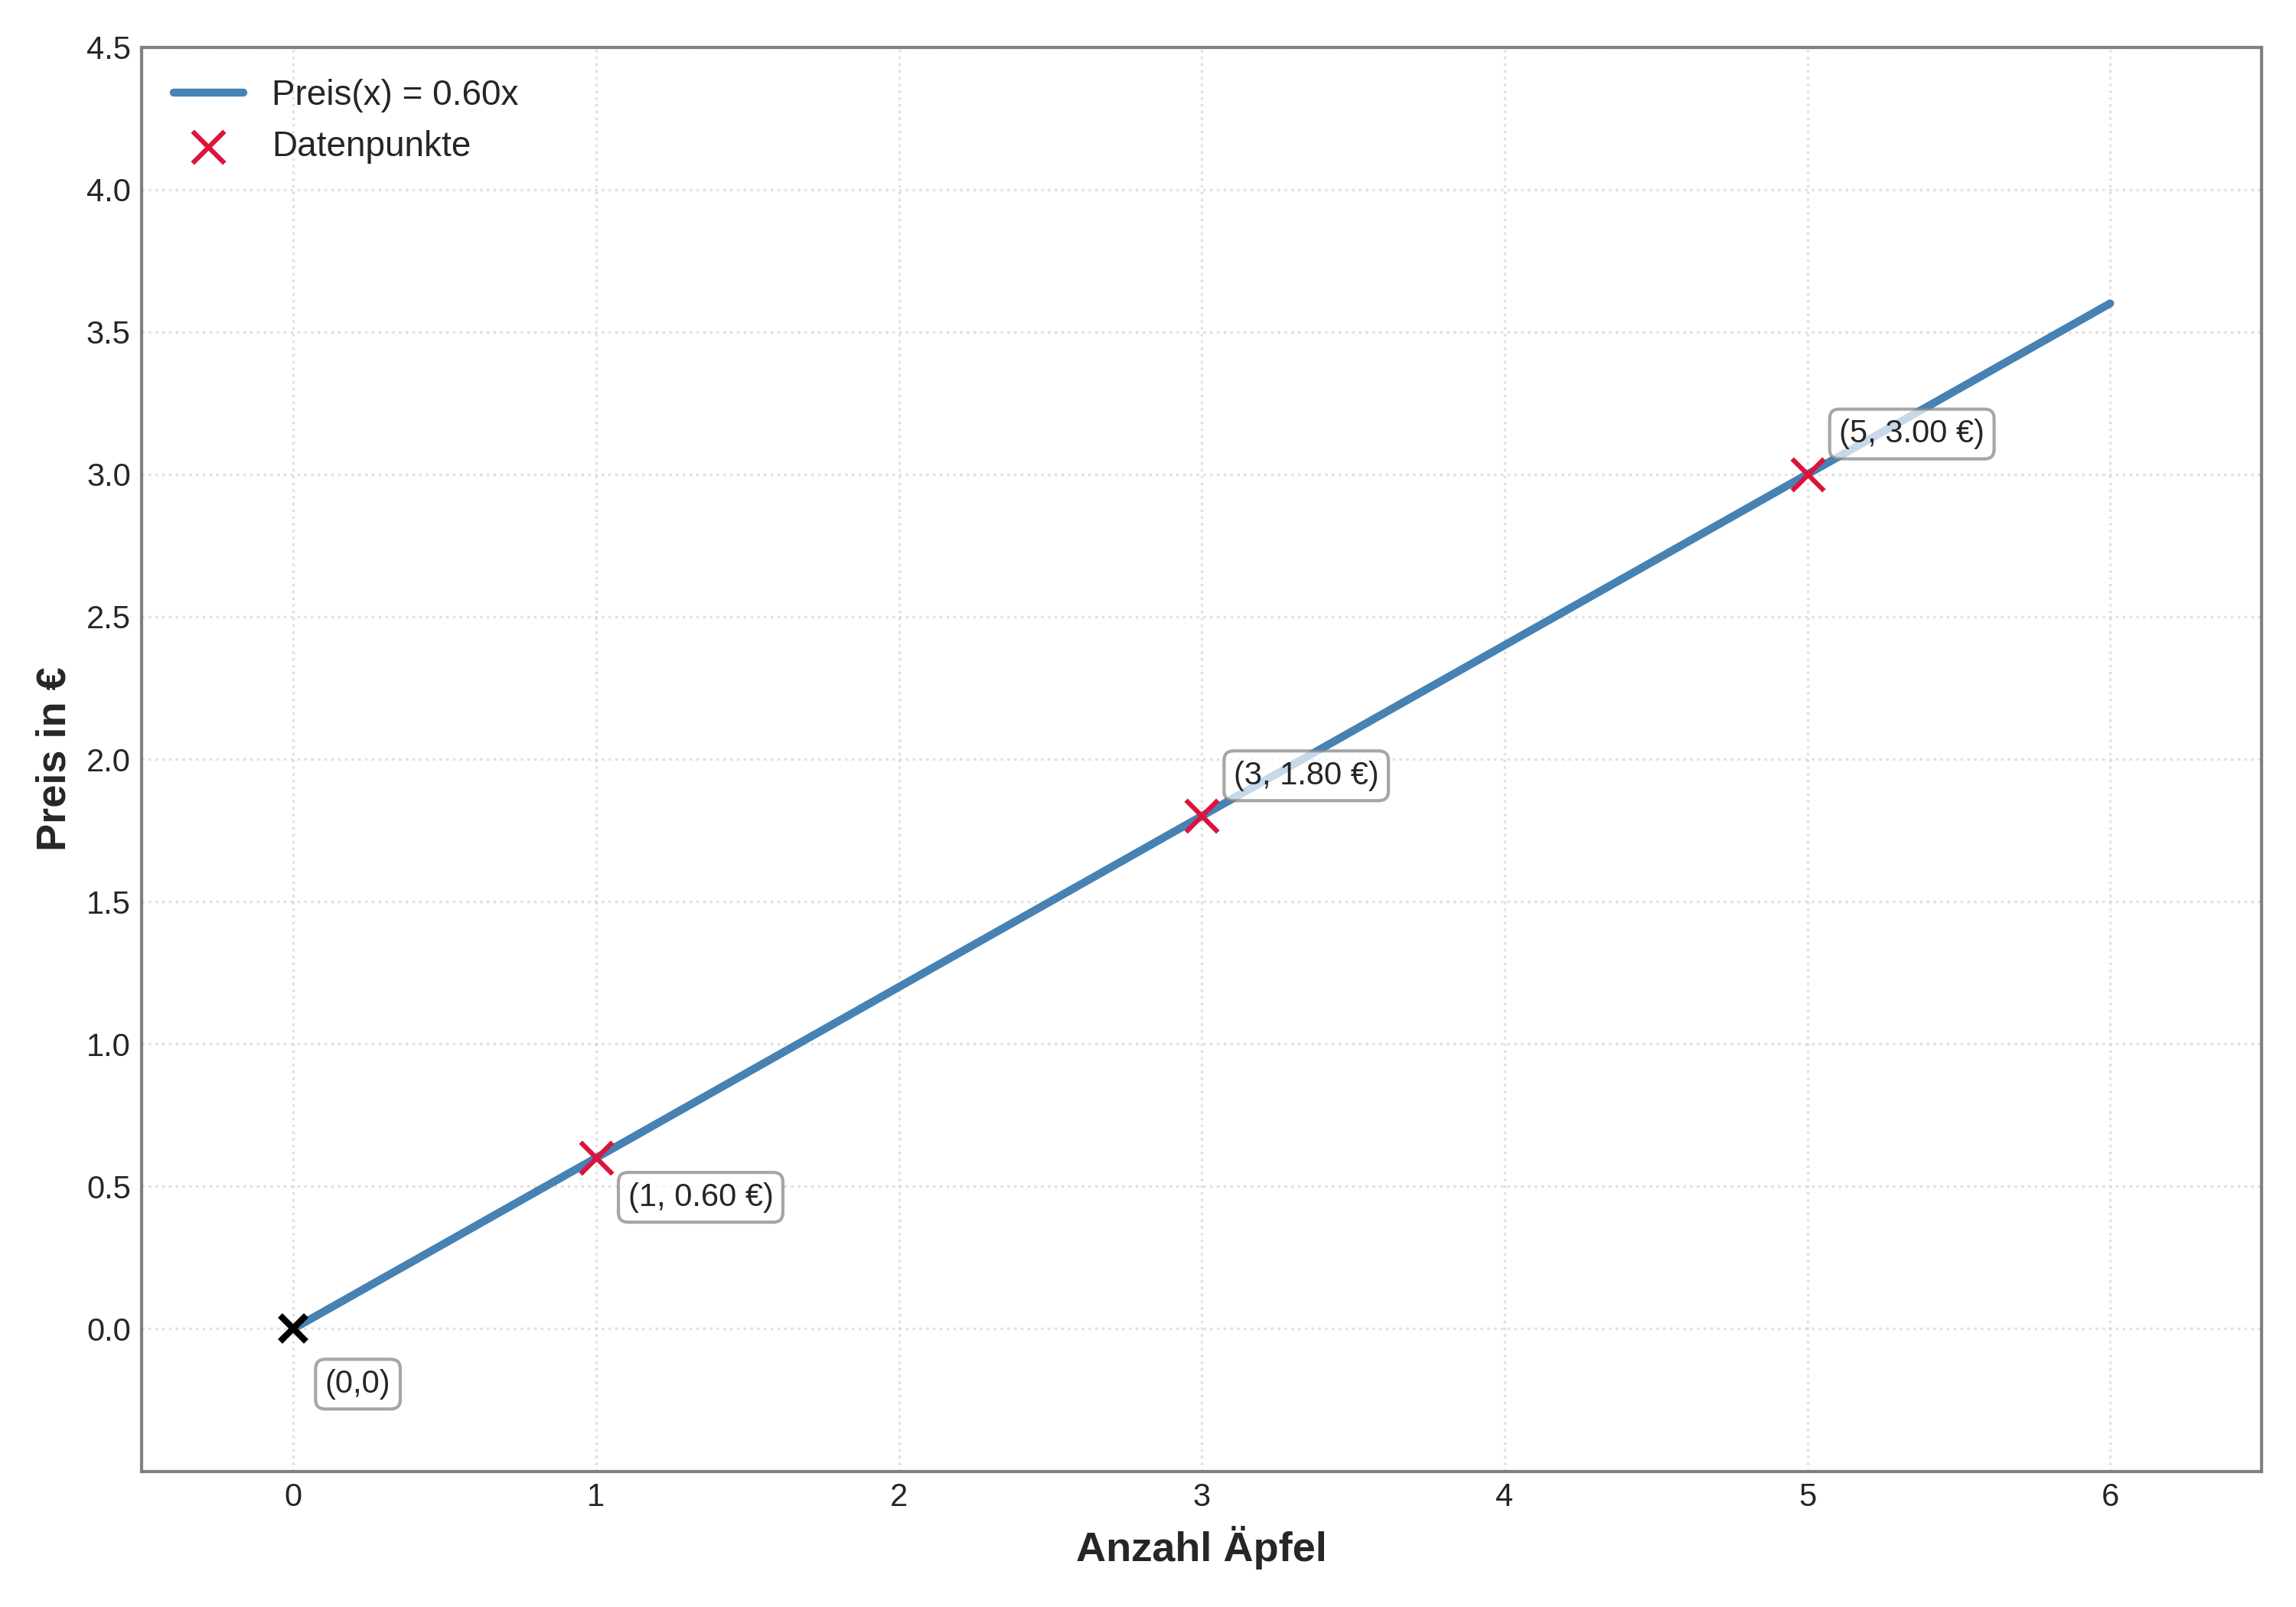
\includegraphics[width=0.8\textwidth]{grafiken/Dreisatz_Apfelpreis_Funktion.png}
    \caption{Preis für Äpfel als lineare Funktion} % \captionof{figure} wird zu \caption innerhalb der figure-Umgebung
    \label{fig:dreisatz_apfel_funktion}
\end{figure}

Dieser Übergang vom konkreten Rechnen mit dem Dreisatz zur abstrakteren Darstellung mit Funktionen ist ein wichtiger Schritt in der Mathematik. Im nächsten Kapitel schauen wir uns lineare Funktionen noch viel genauer an!